%%%%%%%%%%%%%%%%%%%%%%%%%%%%%%%%%%%%%%%%%%%%%%%%%%%%%
% Primary document settings
%%%%%%%%%%%%%%%%%%%%%%%%%%%%%%%%%%%%%%%%%%%%%%%%%%%%%

\documentclass[aspectratio=169,12pt]{beamer}

\usepackage{ifxetex,ifluatex}
\ifnum 0\ifxetex 1\fi\ifluatex 1\fi=0 % if pdftex
  \usepackage[T1]{fontenc}
  \usepackage[utf8]{inputenc}
  \usepackage{textcomp} % provide euro and other symbols
\else % if luatex or xetex
  \usepackage{unicode-math}
  \defaultfontfeatures{Scale=MatchLowercase}
  \defaultfontfeatures[\rmfamily]{Ligatures=TeX,Scale=1}

\usepackage[
    backend=biber,
    natbib=true,
    style=authoryear-comp,
    %bibstyle=authoryear,
    %autocite=footnote,
    %style=authoryear,
    sorting=nyt,
    %sortlocale=de_DE,
    sortlocale=en_US,
    url=false,
    doi=true,
]{biblatex}

\addbibresource{references.bib}
\addbibresource{library.bib}

\usepackage{fancyqr}

%%%%%%%%%%%%%%%%%%%%%%%%%%%%%%%%%%%%%%%%%%%%%%%%%%%%%%%%%%%%%%
% Extra stuff for Rmarkdown to work (code blocks)
%%%%%%%%%%%%%%%%%%%%%%%%%%%%%%%%%%%%%%%%%%%%%%%%%%%%%%%%%%%%%%
\providecommand{\tightlist}{%
  \setlength{\itemsep}{2pt}\setlength{\parskip}{0pt}}

\usepackage{graphicx}
\makeatletter
\def\maxwidth{\ifdim\Gin@nat@width>\linewidth\linewidth\else\Gin@nat@width\fi}
\def\maxheight{\ifdim\Gin@nat@height>\textheight\textheight\else\Gin@nat@height\fi}
\makeatother
% Scale images if necessary, so that they will not overflow the page
% margins by default, and it is still possible to overwrite the defaults
% using explicit options in \includegraphics[width, height, ...]{}
\setkeys{Gin}{width=\maxwidth,height=\maxheight,keepaspectratio}
% Set default figure placement to htbp
\makeatletter
\def\fps@figure{htbp}
\makeatother

%%%%%%%%%%%%%%%%%%%%%%%%%%
% kableExtra stuff (tables)
%%%%%%%%%%%%%%%%%%%%%%%%%%
\usepackage{booktabs}
\usepackage{longtable}
\usepackage{array}
\usepackage{multirow}
\usepackage{xcolor}
\usepackage{wrapfig}
\usepackage{float}
\usepackage{colortbl}
\usepackage{pdflscape}
\usepackage{tabu}
\usepackage{threeparttable}
\usepackage{threeparttablex}
\usepackage[normalem]{ulem}
\usepackage{makecell}

%%%%%%%%%%%%%%%%%%%%%%%%%%
% Main document
%%%%%%%%%%%%%%%%%%%%%%%%%%

\usetheme[fira]{BIPS}
%\usetheme[german]{BIPS}  % for the German version
%\usetheme[fira]{BIPS} % English with the Fira font
%\usetheme[german,fira]{BIPS} % German with the Fira font

% Note that for the Fira font, you need to use
% XeLaTeX instead of pdfLaTeX. You can find this in
% most interfaces

\title{A Large-Scale Neutral Comparison Study\\
of Survival Models}
\subtitle{}
\author{Burk, L.\inst{1,2,3,4} \and Zobolas, J.\inst{5} \and Bischl,
B.\inst{2,4} \and Bender, A.\inst{2,4} \and Wright, M.
N.\inst{1,3} \and Lang, M.\inst{6} \and Sonabend, R.\inst{7, 8}}
\date{}
\contactauthor{Lukas Burk}
\occasion{Biometric Colloquium --- March 1st, 2024}
\email{burk@leibniz-bips.de}
\institute{\textsuperscript{1}Leibniz Institute for Prevention Research
and Epidemiology -- BIPS \and \textsuperscript{2}LMU Munich
\quad \textsuperscript{3}University of
Bremen \and \textsuperscript{4}Munich Center for Machine Learning
(MCML) \and \textsuperscript{5}University of Oslo
\quad \textsuperscript{6} TU Dortmund \and \textsuperscript{7}OSPO Now
\quad \textsuperscript{8}Imperial College, London}

%\author[Burk, Bender, Wright]% (optional, for multiple authors)
%{Lukas Burk\inst{1} \and Andreas Bender\inst{2,3} \and Marvin N. Wright\inst{1}}

%\institute%
%{
%  \inst{1}%
%  Leibniz Institute for Prevention Research and Epidemiology -- BIPS\\
%  \inst{2}%
%  LMU Munich\\
  %\and
%  \inst{3}%
%  Munich Center for Machine Learning (MCML)
%}

%%% Title Page
\setbeamertemplate{title page}{
	\usebeamercolor{title page}
	\begin{tikzpicture}
		\useasboundingbox (1,0) rectangle (\the\paperwidth,\the\paperheight);
		\node[font=\usebeamerfont{title}, color=BIPSBlue, text width=14cm, align=center] at (\paperwidth*.5,7) {\inserttitle} ;
		% \node[align=center, font=\usebeamerfont{subtitle}, color=BIPSBlue] at (\paperwidth*.5, 5.5) {\insertsubtitle};
		\node[align=center, font=\usebeamerfont{author}, color=BIPSBlue] at (\paperwidth*.5, 5) {\insertauthor};
		\node[align=center, font=\usebeamerfont{institute}, color=BIPSTextGray] at (\paperwidth*.5, 3) {\textsuperscript{1}Leibniz
Institute for Prevention Research and Epidemiology --
BIPS \\ \textsuperscript{2}LMU Munich
\quad \textsuperscript{3}University of
Bremen \\ \textsuperscript{4}Munich Center for Machine Learning
(MCML) \\ \textsuperscript{5}University of Oslo
\quad \textsuperscript{6} TU Dortmund \\ \textsuperscript{7}OSPO Now
\quad \textsuperscript{8}Imperial College, London};
		\node[align=center, font=\usebeamerfont{date}, color=BIPSTextGray] at (\paperwidth*.5, 1.5) {\insertdate};
		\node[align=center, font=\usebeamerfont{date}, color=BIPSTextGray] at (\paperwidth*.5, 1) {Biometric
Colloquium --- March 1st, 2024};
	\end{tikzpicture}
}


%\author{Lukas Burk\inst{1} \and Andreas Bender\inst{2}\inst{3} \and Marvin N. Wright\inst{1}}
% Affiliations
%\institute[short]{\inst{1} Leibniz Institute for Prevention Research and Epidemiology - BIPS \\ \inst{2} LMU Munich \\ \inst{3} Munich Center for Machine Learning (MCML)}

\begin{document}
\addtocounter{framenumber}{-1}
\frame{\maketitle}

% \setcounter{framenumber}{1}


\begin{frame}{Introduction}
\phantomsection\label{introduction}
\begin{itemize}[<+->]
\tightlist
\item
  There are many survival learners (``models'') to choose from
\item
  Advantages and disadvantages often unclear, specific to setting
\item
  Various comparisons exist in literature
\item
  Limited scope (learners, tasks, evaluation measures)
\item
  Focus on individual / new method \(\Rightarrow\) no neutral comparison
\item
  No (or limited) quantitative comparison
\end{itemize}

\pause

\vspace{1em}

\(\Rightarrow\) Needs \emph{comprehensive comparison}!
\end{frame}

\begin{frame}{Quick Summary}
\phantomsection\label{quick-summary}
\begin{itemize}
\tightlist
\item
  \textbf{32} tasks
\item
  \textbf{18} learners
\item
  \textbf{2} tuning measures
\item
  \textbf{9} evaluation measures
\end{itemize}

\vspace{1em}

\pause

\begin{itemize}
\tightlist
\item
  \textbf{Large-scale} \(\Rightarrow\) Generalizability
\item
  \textbf{Neutral} \(\Rightarrow\) Fair comparison
\end{itemize}

\pause

\vspace{1em}

\(\Rightarrow\) The \emph{largest survival benchmark} to date as far as
we know
\end{frame}

\begin{frame}{Scope}
\phantomsection\label{scope}
The \emph{``Standard Setting''}:

\vspace{1em}

\begin{itemize}
\tightlist
\item
  Single-event outcome: \(\delta_i \in \{0, 1\}\)
\item
  Low-dimensional: \(2 \leq p < n\)
\item
  No time-varying covariates
\item
  Right-censoring only
\item
  At least 100 observed events
\end{itemize}
\end{frame}

\begin{frame}{Tasks}
\phantomsection\label{tasks}
\textbf{32} tasks collected from R packages on CRAN

\begin{table}
\centering
\begin{tabular}[t]{>{}lrrrrr}
\toprule
 & Minimum & q25\% & Median & q75\% & Maximum\\
\midrule
\textbf{N} & 137 & 446 & 820 & 2378 & 52410\\
\textbf{p} & 2 & 4 & 5 & 7 & 25\\
\textbf{Observed Events} & 101 & 194 & 323 & 699 & 5616\\
\textbf{Cens. \%} & 6 & 32 & 48 & 74 & 95\\
\bottomrule
\end{tabular}
\end{table}
\end{frame}

\begin{frame}[fragile]{Learners}
\phantomsection\label{learners}
\textbf{18} learners implemented in R and available via the
\texttt{mlr3} \footnote<.->{\textcite{pkgmlr3}} framework

\vspace{1em}

\pause

\begin{itemize}[<+->]
\tightlist
\item
  \textbf{Baseline}: Kaplan-Meier \& Nelson-Aalen, Akritas
\item
  \textbf{Classical}: Cox, penalized (L1,L2), parametric (AFT)
\item
  \textbf{Trees}: Individuals and ensembles
\item
  \textbf{Boosting}: Gradient- and likelihood-based
\item
  \textbf{Other}: SVM
\end{itemize}
\end{frame}

\begin{frame}{List of Learners (Baseline, Classical)}
\phantomsection\label{list-of-learners-baseline-classical}
\begin{table}
\centering
\begin{tabular}[t]{>{}ll>{}l}
\toprule
Name & Abbreviation & Package\\
\midrule
\textbf{Kaplan-Meier} & KM & \ttfamily{survival}\\
\textbf{Nelson-Aalen} & NA & \ttfamily{survival}\\
\textbf{Akritas} & AK & \ttfamily{survivalmodels}\\
\midrule
\textbf{Cox Regression} & CPH & \ttfamily{survival}\\
\textcolor[HTML]{1763AA}{\textbf{Penalized Cox Regression (L1, L2)}} & \textcolor[HTML]{1763AA}{GLM} & \textcolor[HTML]{1763AA}{\ttfamily{glmnet}}\\
\textcolor[HTML]{1763AA}{\textbf{Penalized Cox Regression (L1, L2)}} & \textcolor[HTML]{1763AA}{Pen} & \textcolor[HTML]{1763AA}{\ttfamily{penalized}}\\
\textbf{Parametric (AFT)} & Par & \ttfamily{survival}\\
\textbf{Flexible Parametric Splines} & Flex & \ttfamily{flexsurv}\\
\midrule
\textbf{Survival SVM} & SSVM & \ttfamily{survivalsvm}\\
\bottomrule
\end{tabular}
\end{table}
\end{frame}

\begin{frame}{List of Learners (Trees, Boosting)}
\phantomsection\label{list-of-learners-trees-boosting}
\begin{table}
\centering
\begin{tabular}[t]{>{}ll>{}l}
\toprule
Name & Abbreviation & Package\\
\midrule
\textbf{Decison Tree} & RRT & \ttfamily{rpart}\\
\textcolor[HTML]{1763AA}{\textbf{Random Survival Forest}} & \textcolor[HTML]{1763AA}{RFSRC} & \textcolor[HTML]{1763AA}{\ttfamily{randomForestSRC}}\\
\textcolor[HTML]{1763AA}{\textbf{Random Survival Forest}} & \textcolor[HTML]{1763AA}{RAN} & \textcolor[HTML]{1763AA}{\ttfamily{ranger}}\\
\textbf{Conditional Inference Forest} & CIF & \ttfamily{partykit}\\
\textbf{Oblique RSF} & ORSF & \ttfamily{aorsf}\\
\midrule
\textbf{Model-Based Boosting} & MBO & \ttfamily{mboost}\\
\textbf{Likelihood-Based Boosting} & CoxB & \ttfamily{CoxBoost}\\
\textcolor[HTML]{1763AA}{\textbf{Gradient Boosting (Cox objective)}} & \textcolor[HTML]{1763AA}{XGBCox} & \textcolor[HTML]{1763AA}{\ttfamily{xgboost}}\\
\textcolor[HTML]{1763AA}{\textbf{Gradient Boosting (AFT objective)}} & \textcolor[HTML]{1763AA}{XGBAFT} & \textcolor[HTML]{1763AA}{\ttfamily{xgboost}}\\
\bottomrule
\end{tabular}
\end{table}
\end{frame}

\begin{frame}{Tuning}
\phantomsection\label{tuning}
\begin{itemize}[<+->]
\tightlist
\item
  Tuning spaces discussed with learner authors
\item
  \textbf{Resampling}: Nested cross-validation (5-fold outer, 3-fold
  inner)
\item
  \textbf{Strategy}: Random Search
\item
  \textbf{Budget}: Tuning stopped if \emph{either} is reached

  \begin{enumerate}[<+->]
  \tightlist
  \item
    Number of evaluations:
    \(n_{\text{evals}} = n_{\text{parameters}} \times 50\)
  \item
    Tuning time of 150 hours (\(6 \tfrac{1}{4}\) days)
  \end{enumerate}
\end{itemize}
\end{frame}

\begin{frame}{Evaluation}
\phantomsection\label{evaluation}
\begin{itemize}[<+->]
\tightlist
\item
  Main Results:

  \begin{itemize}[<+->]
  \tightlist
  \item
    Friedman rank sum tests
  \item
    Critical difference plots\footnote<.->{\textcite{Demsar2006}} based
    on Bonferroni-Dunn tests
  \end{itemize}
\item
  3 types of metrics: Discrimination, Calibration, \emph{Scoring Rules}
\item
  Tuned on 2 different measures

  \begin{itemize}[<+->]
  \tightlist
  \item
    Harrell's C (Discrimination)
  \item
    Right-Censored Log Loss (Scoring Rule)
  \end{itemize}
\end{itemize}
\end{frame}

\section{Results}\label{results}

\begin{frame}{Boxplot (Harrel's C, higher is better)}
\phantomsection\label{boxplot-harrels-c-higher-is-better}
\begin{center}
\includegraphics{01MAR24_Lukas_Burk_files/figure-beamer/boxplot-harrell-1.png}
\end{center}
\end{frame}

\begin{frame}{Boxplot (IBS, lower is better)}
\phantomsection\label{boxplot-ibs-lower-is-better}
\begin{center}
\includegraphics{01MAR24_Lukas_Burk_files/figure-beamer/boxplot-ibs-rcll-full-1.png}
\end{center}
\end{frame}

\begin{frame}{Boxplot (IBS, truncated)}
\phantomsection\label{boxplot-ibs-truncated}
\begin{center}
\includegraphics{01MAR24_Lukas_Burk_files/figure-beamer/boxplot-ibs-rcll-reduced-1.png}
\end{center}
\end{frame}

\begin{frame}{Critical Difference: Bonferroni-Dunn (Harrell's C)}
\phantomsection\label{critical-difference-bonferroni-dunn-harrells-c}
\begin{center}
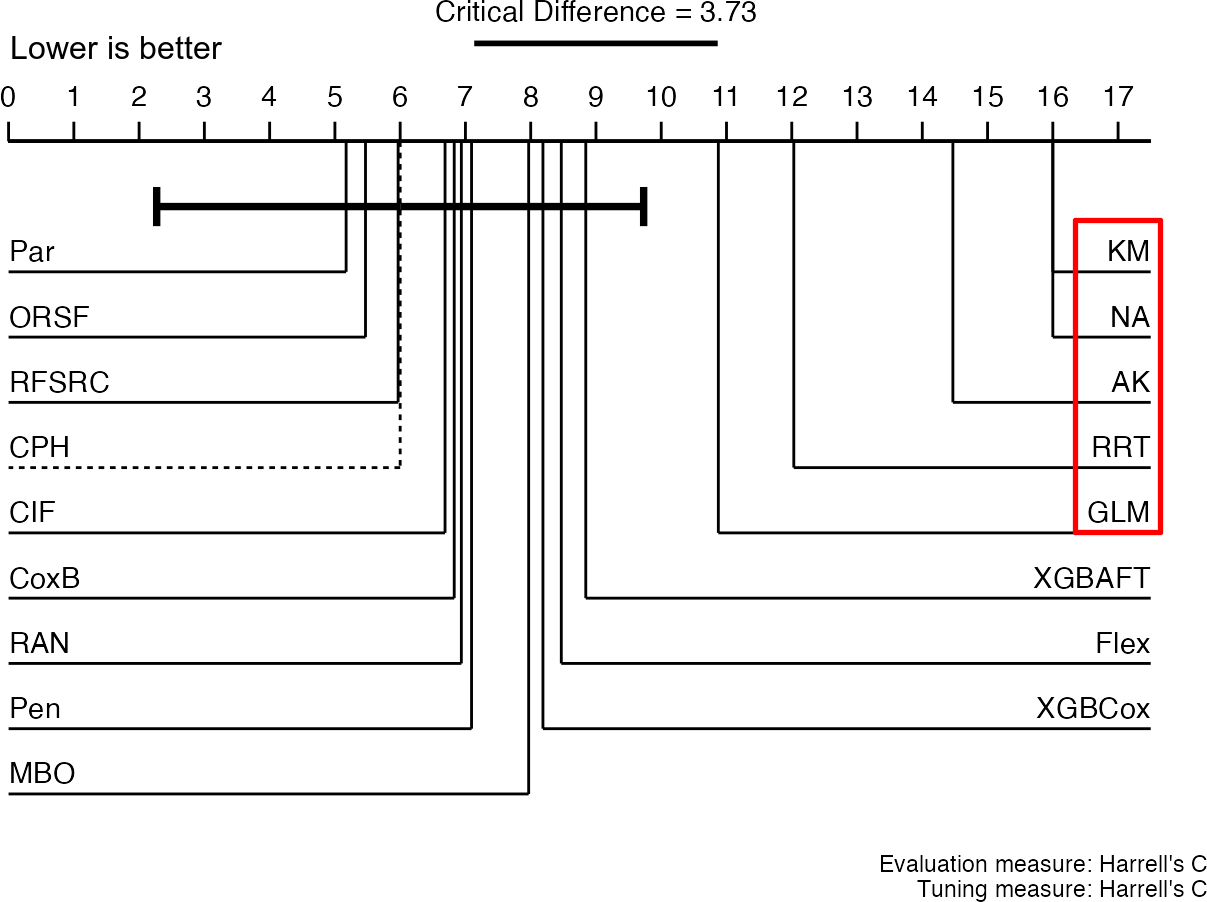
\includegraphics[width=4.02in,height=0.75\textheight]{img/critical-difference-baseline-diff-harrell-c-1-annotated.png}
\end{center}
\end{frame}

\begin{frame}{Critical Difference: Bonferroni-Dunn (IBS/RCLL)}
\phantomsection\label{critical-difference-bonferroni-dunn-ibsrcll}
\begin{center}
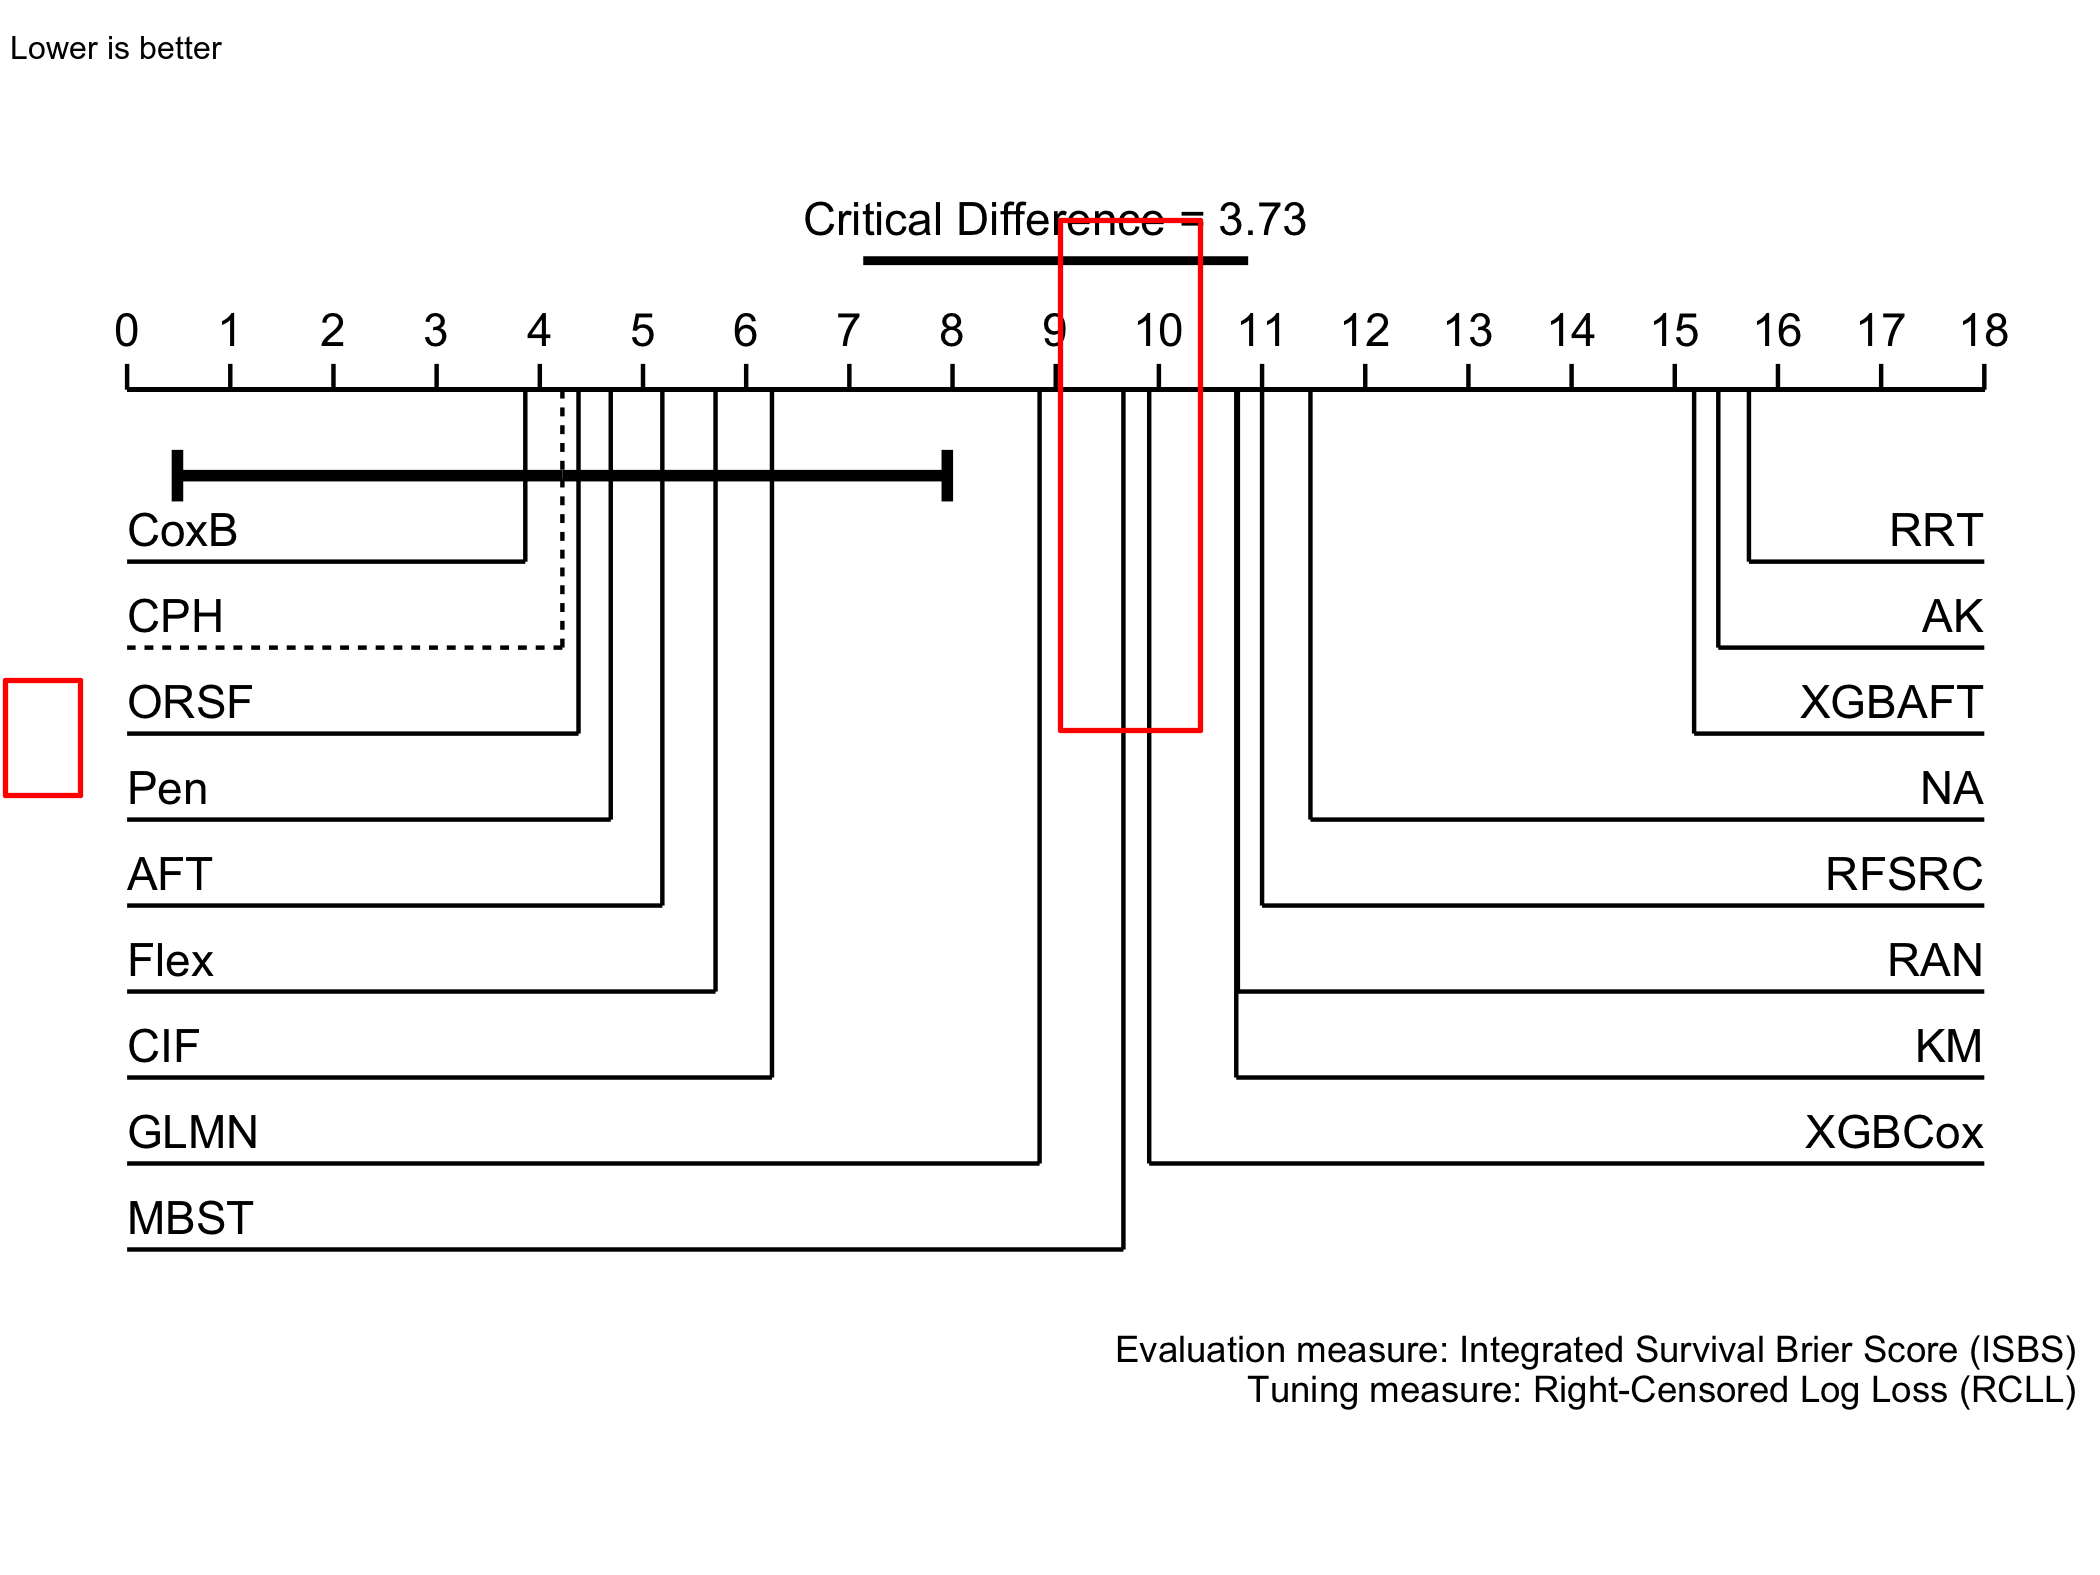
\includegraphics[width=4.14in,height=0.75\textheight]{img/critical-difference-baseline-diff-rcll-7-annotated.png}
\end{center}
\end{frame}

\begin{frame}{Closing Remarks}
\phantomsection\label{closing-remarks}
\begin{itemize}[<+->]
\tightlist
\item
  Only computationally feasible due to resources of ARCC \footnote<.->{Advanced
    Research Computing Center, Beartooth Computing Environment,
    University of Wyoming.}

  \begin{itemize}[<+->]
  \tightlist
  \item
    Sequential runtime \(\approx\) 18 years
  \item
    Effective runtime \(\approx\) 32 days
  \end{itemize}
\item
  Experimental design is not perfect, but it was \emph{possible} to
  conduct
\item
  Results still need processing, checking, \ldots{}
\item
  \textbf{Preliminary conclusion}: Cox regression --- hard to beat since
  1972!
\end{itemize}
\end{frame}

%%% Final slide with contact information
\thanksframe{Thank you for your attention!}

%%% bib?
\begin{frame}[allowframebreaks]{References}
  \printbibliography[heading=none]
\end{frame}

\end{document}
